
\textbf{\underline{В первой главе}} представлены обзоры и анализы областей, которые необходимы для решения поставленных научных задач.

Была проведена классификация машин, использующих ноги в качестве движителя. По результатам классификации объектом исследования является многоногая шагающая машина с движителями циклического действия. Изучив данный класс машин были осмыслены габаритные и структурные особенности этих роботов.

Так как основным местом применения разработанных методов предполагается исследование пещер роботами, то были рассмотрены типы роботов и робототехнических систем, которые могут использоваться для изучения поверхности пещер.

Для решения задачи определения геометрических и физико-механических свойств пройденной поверхности необходимо понимать в каких условиях будет использоваться робот: типы препятствий и размеры. В пещерах встречаются следующие типы поверхностей: твердые породы, прочные (мрамор), мягкие (мел, известняк); сыпучие грунты (песок); водные преграды (лужи, бассейны); скользкие и упругие поверхности (мох, плесень); пластинчатые (земля). Было решено сделать упор на твердые, упругие и пластинчатые поверхности. Длины многих пещер измеряются километрами, а их габариты очень сильно варьируются от нескольких сантиметров, до многих километров в ширину.

Задача определения геометрических свойств объекта является частью Mapping из  класса методов Simultaneous Localization and Mapping (SLAM). Рассмотрев различные варианты, задача локализации решалась с помощью маяков или ToF камеры, а для построения карты был разработан свой метод.

Проведен обзор алгоритмов триангуляции, так как данный метод лёг в основу определения геометрических свойств объекта. Было решено модифицировать 2D триангуляцию Делоне для вогнутых оболочек.

Рассматривались различные алгоритмы и средства определения физико-механических свойств поверхности. Было решено выбрать главным сенсором --- датчик силы, установленный на ногу робота, но также собирать дополнительные данные об угловой скорости и моменте на моторе.

Для решения задачи оптимизации количества ног робота, необходимо генерировать семейства поверхностей с одинаковой сложностью. Поиск различных вариантов привел к выбору подхода <<Получение искусственных поверхностей на основе параметров генерации>>, который был модифицирован автором.

На основе литературного обзора было выявлено, что предложенные решения для определения геометрических и физико-механических свойств не встречается в научных публикациях российских и зарубежных авторов.

На основе проведенного анализа, разработана концепция робота \pic{fig:diag_system.png}. Оранжевым цвет --- компоненты системы, которые представляют собой предмет исследования в рамках диссертационной работы. Голубым цветом выделены блоки которые были интегрированы как стандартные средства, без каких-либо существенных доработок.
\begin{figure}[ht!]
    \centering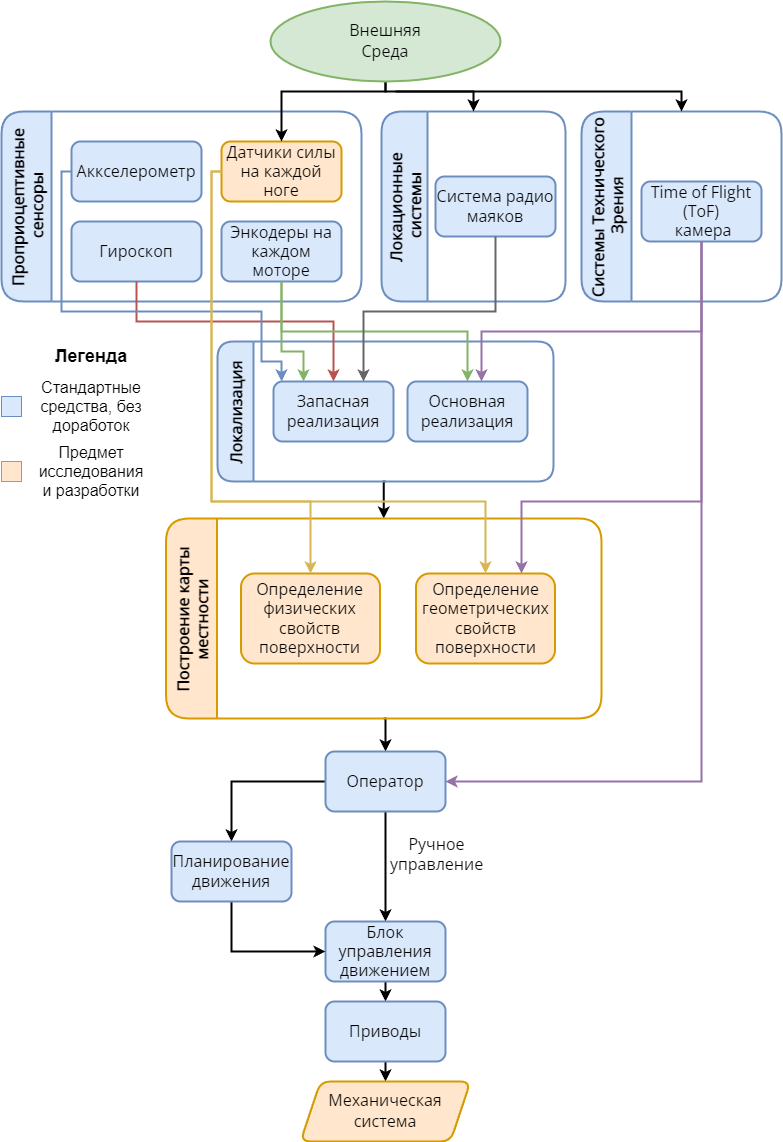
\includegraphics[height=15cm,width=1\textwidth,keepaspectratio]{main_diag.drawio.png}
    \caption{Структурная схема разработанной системы}
    \label{fig:diag_system.png}
\end{figure}


